% !TeX encoding = UTF-8
% !TeX root = V39_Spectroscopy_Rb.tex
% !TeX spellcheck = en_US

\section{Introduction}
This experiment gives us an insight about experimental atom physics and the fundamental of laser physics. We study the principle of a diode laser and the methods how to calibrate one with both an internal and external resonator, the latter set in a Littrow configuration.\\
The goal of this experiment is the spectroscopy of the D2 line $(780,027 \nano\metre)$ of the Rubidium atom, which is present as a gas in a cell.\\
The first step is to conduct an absorption spectroscopy of the Rb gas. Because of the doppler shift, it isn't possible to resolve the hyperfine structure of the D2. This will be solved by using the method of the saturated absorption spectroscopy, for which the experimental setup will be slightly altered. Furthermore, we will improve the former results by performing the frequency modulation spectroscopy.

\newpage
\section{Theory}
The following elaboration of the physical basics is based on  \cite{lit:AK_manual2012} and \cite{lit:SAS}.

\subsection{Diode laser}
\begin{figure}[bh]
	\centering
	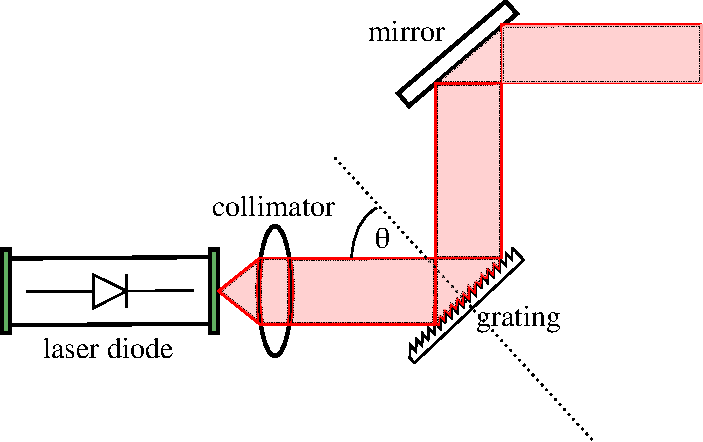
\includegraphics[width=0.8\textwidth]{laser_diode.pdf}
	\caption[Schematic of a diode laser in Littrow configuration]{Schematic setup for a diode laser in Littrow configuration. The angle of the grating is set such that the first diffraction order coincides with the output beam from the laser diode. While all components are fixed here, the collimator and the grating are movable for necessary adjustment of the laser.}
	\label{fig:laser_diode}
\end{figure}

In a diode laser, the pn transition is the active medium. A voltage is applied on the diode to neutralize the internal electrical field and thus the excess electrons of the n-layer are able to recombine with the defect electrons, namely 'holes', of the p-layer. In this process, the electrons total energy decrease. The energy difference between the two levels is emitted as a electromagnetic wave with frequency $\nu=\Delta E/h$, while $h$ is the Planck constant.\\
The two ends of the laser diode form the \emph{internal resonator}. One of the ends is a mirror with a 100\% reflectance, while the other end is a semi-permeable medium, which reflects most of emitted beam and thus works as a laser pump. The electrons in the diode will be excited with the energy they previously emitted, and emit the energy again with the same wavelength, direction and polarization (i.e. stimulated emission). By setting a certain length of the laser diode, you can amplify a particular range of wavelengths. Due to the size of the diode casing, the free spectral range (FSR) is given by
\begin{equation}
\Delta \nu=\frac{c}{2L}.
\end{equation}
For an usual casing with a few millimeters of size for $L$, the FSR is roughly $100\giga\hertz$, while the line width is usually about $100\mega\hertz$ \cite{lit:AK_manual2012}.

For further narrowing of the line width, since it is needed for our spectroscopy, we will use an \emph{external resonator} in Littrow configuration. It consists of the reflective back side of the laser diode and a particular grating being set on an angle (see figure \ref{fig:laser_diode}) such that the first order diffraction beam is reflected back into the diode laser (see \cite{lit:AK_manual2012}). Since the diffraction is wavelength-dependent, we can configure the diode laser as desired. The usual obtained line widths are below $1\mega\hertz$.\\
Taking the gains of all the components into account, we can set the diode laser (see figure~\ref{fig:gain_profiles}) to a certain frequency.
\begin{figure}[h]
	\centering
	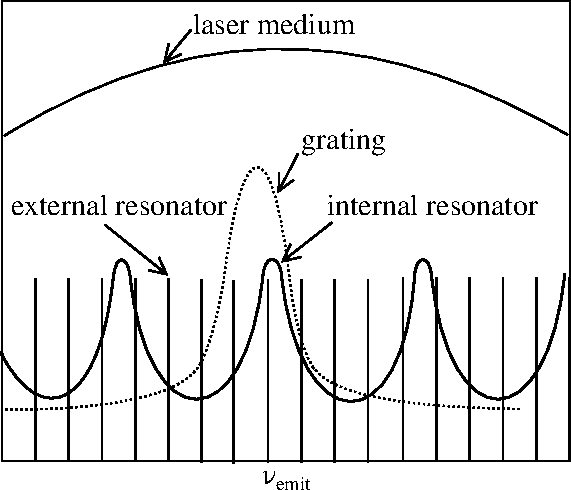
\includegraphics[width=0.8\textwidth]{gain_profile.pdf}
	\caption[Gain profile of a diode laser]{Gain profile of a diode laser. The laser diode contributes to the total profile with its laser medium and the internal resonator. }
	\label{fig:gain_profiles}
\end{figure}

By changing the injection current and the temperature of the laser diode, the gain profile of the internal resonator is shifted due to the altered refractive index. It also sets the frequency range. The external resonator can be modified by altering the angle and the position of the grating. For this, the coarse tuning is done with fine adjustment screws, whereas the fine tuning is done with a piezo. A change in temperature shifts all the profiles, but each with a different shift. To avoid this during the measurements, the temperature has to be necessarily kept constant.

In the \emph{single mode}, only the resonance mode with the highest amplification oscillates and the laser emits quasi-monochromatic light.
When varying the laser cavity during the tuning, the number of waves in the cavity will stay constant for a certain time, but the frequency is changed. If the laser cavity is varied too far, the number of half-wavelengths inside the cavity will jump up or down by one or two. The laser frequency jumps back into the original range. These jumps are called \emph{mode hops}.\\
Before the measurements, the temperature, current, the angle and position of the grating are set so that the spectrum of the measured sample lies within two relatively good mode hops.

\subsection{Structure of the Rb atom}
With quantum mechanics, we can predict the energy levels of the electrons in an atom. For a multi-electron system, those calculations are rather difficult. For this, we use the central field approximation, in which many inter-atom interactions are ignored. Each electron can be described with the quantum numbers $n$ (principle quantum number), $l$ (orbital angular momentum), $m_l$, $s$ (spin) and $m_s$ (further explanations of those numbers can be found in every book about atom physics). The quantum numbers $l$ and $s$ of all electrons can be summed up to the total quantum numbers $L$ and $S$, resulting in the magnitude of the total electronic angular moment $J$, defined as
\begin{align}
J=L+S.
\label{eq:spin_orbit}
\end{align}
The sum of all $l_i$ and $s_i$ over all electrons $i$ in a filled orbit is always equal to zero, thus the total electronic angular momentum corresponds to the one of the single valence electron, making it similar to the hydrogen atom. In the ground state, the orbit of the electron in Rb atom is described as $5{}^2\mathrm{S}_{1/2}$. In a higher state, due to the spin-orbit-coupling described in equation \eqref{eq:spin_orbit}, two different excited states are available: $5{}^2\mathrm{P}_{1/2} (\approx 795 \nano\metre)$ and $5{}^2\mathrm{P}_{3/2} (\approx 780\nano\metre)$. This splitting of the energy levels due to the spin-orbit-coupling is called \emph{fine structure}. In this experiment, because of the applied diode laser, we will only inspect the latter transition with $780\nano\metre$ known as D$_2$ transition.\\
Now we're taking the \emph{spin angular momentum} $I$ of the atom nucleus into account, which depend on the nuclear structure and the isotope. The spin angular momentum is very small compared to the electronic angular momentum, resulting in the small \emph{hyperfine splitting}. We define the \emph{total angular moment} $F$ of the atom as follows:
\begin{align}
F=J+I,
\end{align}
where the magnitude of $F$ goes from $|J-I|$ to $|J+I| $.

From this moment on, we need to consider the fact the Rubidium atom has two natural occurring  isotopes: 72\% abundant $^{85}\text{Rb}$ with $I=5/2$ and 28\% abundant $^{87}\text{Rb}$ with $I=3/2$. This results in two hyperfine levels within $5{}^2\mathrm{S}_{1/2}$ and $5{}^2\mathrm{P}_{1/2}$, while the excited state $5{}^2\mathrm{P}_{1/2}$ splits up into four hyperfine levels.
Figure \ref{fig:hyperfine_85Rb} shows the fine and hyperfine structure of the lowest levels in $^{85}$Rb, where figure \ref{fig:hyperfine_8587Rb} contains the hyperfine structure of both the $^{85}\text{Rb}$ and $^{87}\text{Rb}$ isotope.
\begin{figure}[h]
	\centering
	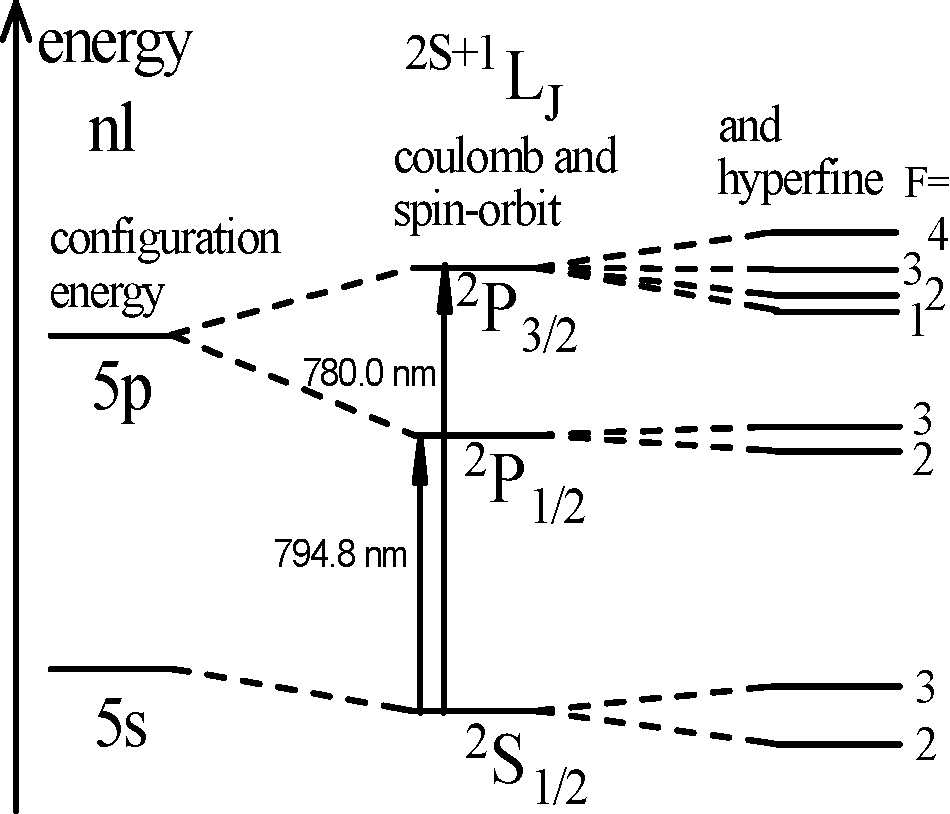
\includegraphics[width=0.8\textwidth]{hyperfine_85Rb.pdf}
	\caption{Energy structure of the lowest levels in $^{85}\text{Rb}$. \cite{lit:SAS}}
	\label{fig:hyperfine_85Rb}
\end{figure}
\begin{figure}[h]
	\centering
	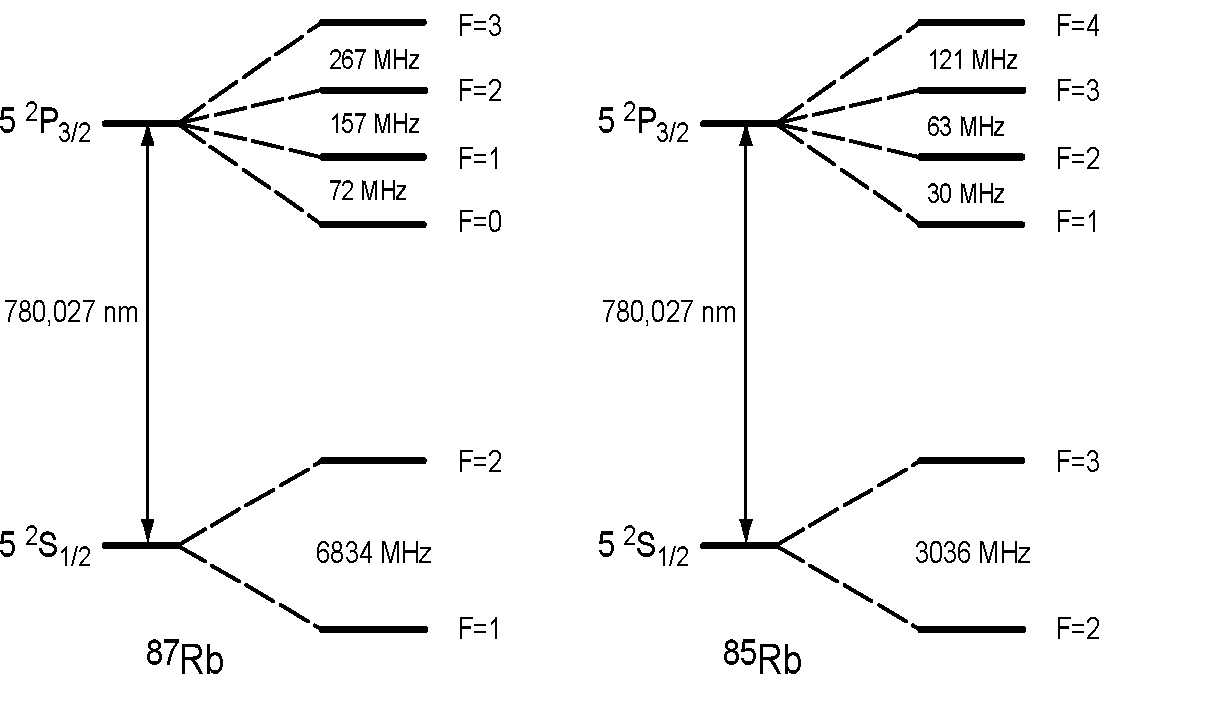
\includegraphics[width=0.8\textwidth]{hyperfine_8587Rb.pdf}
	\caption{Hyperfine structure of both Rb isotopes. \cite{lit:AK_manual2012}}
	\label{fig:hyperfine_8587Rb}
\end{figure}
Concerning the possible transitions, following the selection rule for dipole transitions yields $\Delta F=0,\pm 1$. For each isotope, a total of six transitions are possible, this can be deducted from figure \ref{fig:hyperfine_8587Rb} as well.\\
The hyperfine splitting at the $5{}^2\mathrm{S}_{1/2}$ level is by several orders greater than the one at $5{}^2\mathrm{P}_{3/2}$, and thus can already be detected with the absorption spectroscopy, which is explained in the next section. Figure \ref{fig:hyperfine_ground_8587Rb} shows the relative energy gaps between the hyperfine splitting of both Rb isotopes.
\begin{figure}[h]
	\centering
	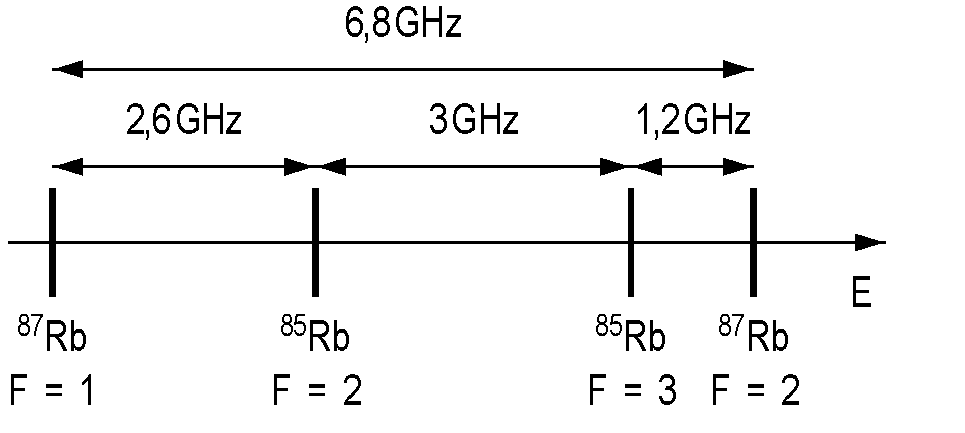
\includegraphics[width=0.8\textwidth]{hyperfine_ground_8587Rb.pdf}
	\caption[Energy gaps in hyperfine structure]{Relative energy gaps between the hyperfine splittings of both Rb isotopes. \cite{lit:AK_manual2012}}
	\label{fig:hyperfine_ground_8587Rb}
\end{figure}

\newpage
\subsection{Laser spectroscopy}
\subsubsection{Absorption spectroscopy}
In the simpliest case of absorption spectroscopy, a gaseous sample of Rb in a cell is hit by a laser beam. We will get the relative absorption by comparing the incident laser intensity to the transmitted intensity detected by a photo diode. \emph{Stimulated absorption} occurs when the frequency of the incident beam becomes resonant with certain transition frequencies, exciting the Rb atoms to a higher level. The gained energy will be emitted \emph{spontaneously} in all directions, thus a fluorescence of the gas and a decline in the transmitted laser intensity are detected.\\
In the reference frame of the atoms, due to the \emph{Doppler effect}, the resonance frequency $\nu_0^\prime$ is shifted such that
\begin{align}
\nu_0^\prime=\nu_0\left(1+\frac{v}{c}\right),
\end{align}
where $v$ is the velocity of the atoms along the laser beam.
%Mean lifetime of a energy state before a transition (Lorentzian curve) mostly ignored resp. overlaid by the Maxwell-Boltzmann distribution
Since we have a thermal gas, the velocities of the gas atoms along the laser beam are Maxwell-Boltzmann distributed as
\begin{align}
P(v)\d v\propto \exp\left(-\frac{mv^2}{2k_B T}\right)\d v
\end{align}
We can conclude the frequency shifts are Maxwell-Boltzmann distributed as well. As a Gaussian distribution, the FWHM $\Delta\nu_{1/2}$ has the shape
\begin{align}
\Delta\nu_{1/2}=2\frac{\nu}{c}\sqrt{\frac{k_B T}{m}2\log 2}
\end{align}
At room temperature, this corresponds to around $4                                                                                                                                                                                                                                                                                                               00\mega\hertz$. The hyperfine splittings of the P levels can't be resolved like this, only the hyperfine splittings of the S levels are visible (see figure \ref{fig:abs_spec}).
\begin{figure}[h]
	\centering
	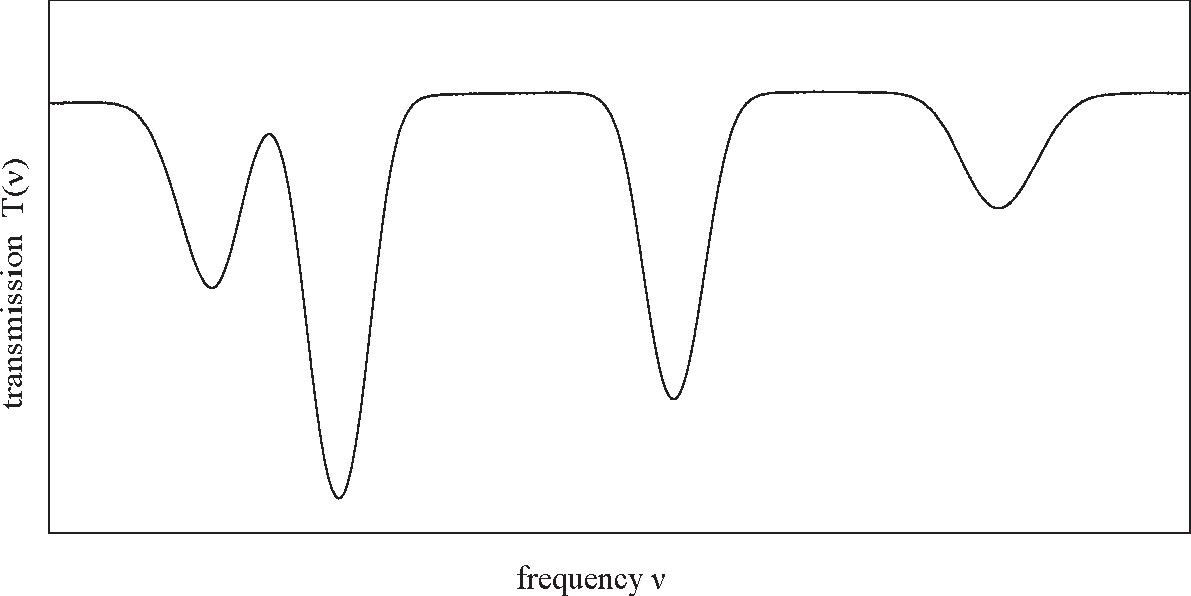
\includegraphics[width=0.8\textwidth]{abs_spec.pdf}
	\caption[Transmission spectrum of the D2 line]{Transmission spectrum of the D2 line. The hyperfine splittings of the S levels are visible. \cite{lit:AK_manual2012}}
	\label{fig:abs_spec}
\end{figure}

\newpage
\subsubsection{Saturated absorption spectroscopy}
\enlargethispage{4em}
In this spectroscopy, the incident beam will be split into two beams with different intensities. The schematic of the setup is shown in figure \ref{fig:setup_abs}. They are focused on the Rb cell from opposite directions. The partial beam with the stronger intensity is the \emph{pump beam}, the weaker one is the \emph{probe beam}. With the pump beam, atoms in the gas cell are excited to a higher level. The probe beam is used to detect the absorption by the atoms, since it isn't absorbed by the atoms which has already been excited by the pump beam. If the atom interacts with both opposing beams, the transmission ratio increases. Due to the doppler shift in two opposing directions, in a two-level-system, this interaction with both beams only occur for atoms with the velocity $v=0$ with respect to the beam direction. The absorption spectrum shows a \emph{Lamb-dip} at $\nu_0$ (see figure \ref{fig:lamb-dip}).

\begin{figure}[h]
	\centering
	\vspace{-3ex}
	\begin{subfigure}{0.45\textwidth}
		\centering
		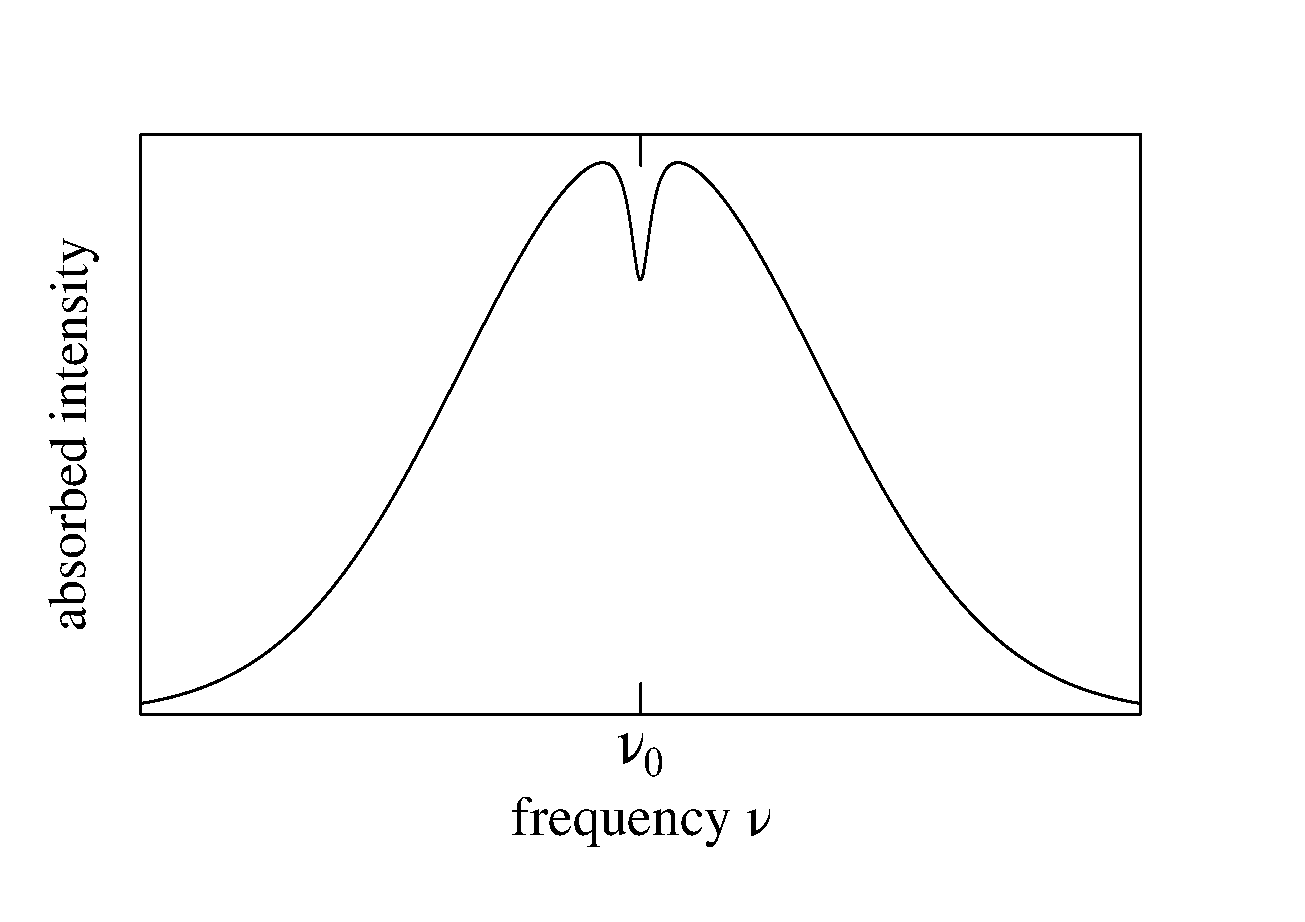
\includegraphics[width=\textwidth]{lamb-dip.pdf}
		\vspace{-2em}
		\caption{Lamb-dip}
		\label{fig:lamb-dip}
	\end{subfigure}
	\hfill
	\begin{subfigure}{0.45\textwidth}
		\centering
		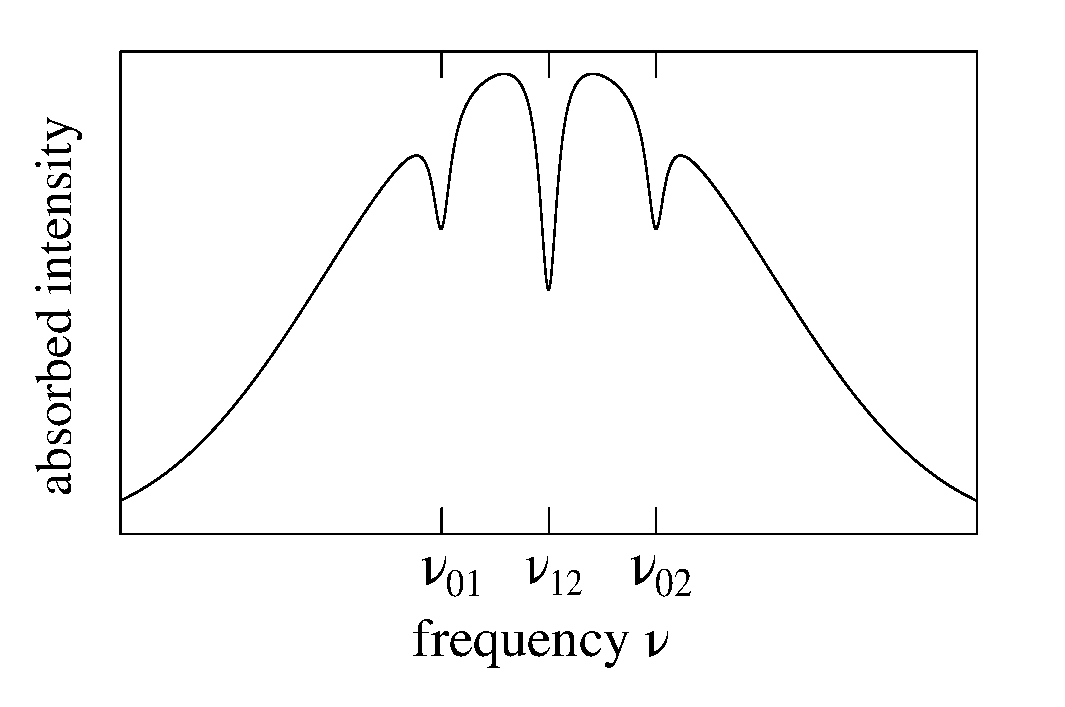
\includegraphics[width=\textwidth]{crossover.pdf}
		\vspace{-2em}
		\caption{Lamb-dips and crossover}
		\label{fig:crossover}
	\end{subfigure}
	\caption[Saturated Absorption Spectroscopy]{Saturated Absorption Spectroscopy: Absorption spectrum of the probe beam for a two-level-system (a) and for a three-level-system (b).}
	\vspace{-1ex}
\end{figure}
In a multi-level system, as the Rb atom is, we also observe another lamb-dips within a absorption range (see figure \ref{fig:crossover}). This is due to \emph{crossover} resonances between two different transitions. The reason is the resonance of the doppler shifts of two atomic transitions. Since the doppler shifts are opposed to each other, this resonance is set in the midst of the two associated transitions.
Figure \ref{fig:sat_abs_spec} shows the saturated absorption spectrum of the D2 line.
\begin{figure}[h]
	\centering
	\vspace{-1em}
	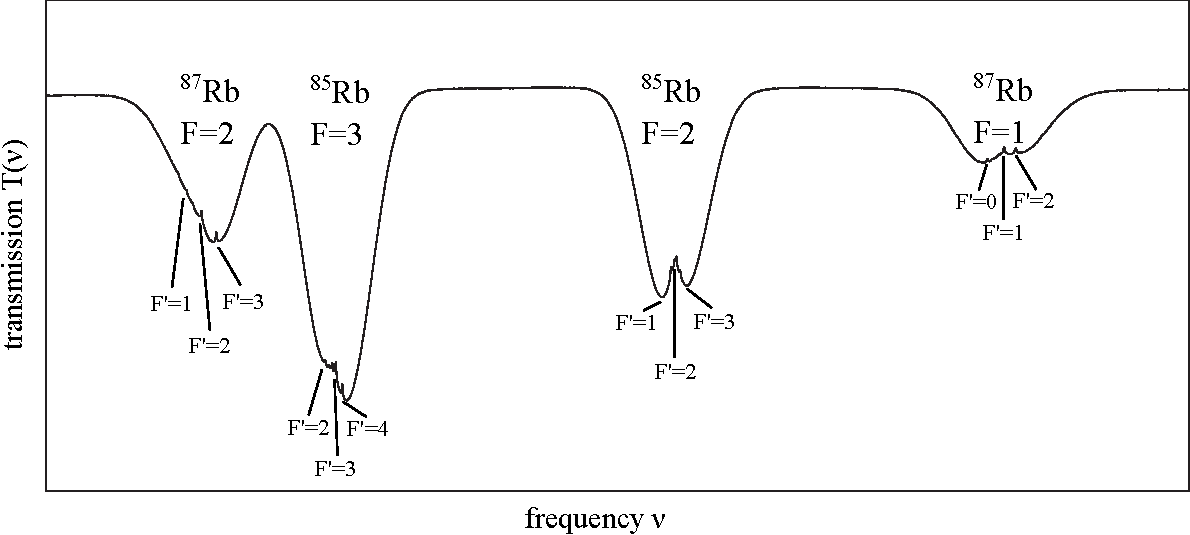
\includegraphics[width=0.8\textwidth]{sat_abs_spec.pdf}
	\caption[Saturated absorption spectrum of the D2 line]{Saturated absorption spectrum of the D2 line. On each doppler broadened base the lamb-dips and crossover resonances can be seen. \cite{lit:AK_manual2012}}
	\label{fig:sat_abs_spec}
	\vspace{-3em}
\end{figure}

\newpage
\subsubsection{Frequency modulation spectroscopy}
In opposite to the two former spectroscopy methods, this FM spectroscopy works with modulating the laser frequency. This will be achieved by modulating the injection current with a periodic signal. The transmitted signal from the probe beam - as before - will be captured by a photodiode and will be processed through a phase detector and a low-pass filter. By demodulating the processed signal turns out to be the derivative of the saturated absorption spectroscopy signal. This is showed as follows (based on \cite{lit:mpi_FM_spec}):\\
We consider the emitted beam with angular velocity $\omega_T$ and modulate the angular velocity with a periodical term. The electrical field component of the beam at a fixed spatial point is
\begin{align}
E(t)=E_0\exp\left(\mathrm{i}\omega_T t+\mathrm{i}M\sin(\omega_M t)\right)+c.c.,
\end{align}
where $M$ is the \emph{modulation index}. If $M\ll 1$, we can use the Taylor series and approximate $E(t)$ such that
\begin{align}
E(t)=E_0\left(\exp(\mathrm{i}\omega_T t)-\frac{M}{2}\exp(\mathrm{i}(\omega_T-\omega_M)t)+\frac{M}{2}\exp(\mathrm{i}(\omega_T+\omega_M)t\right)+c.c.
\end{align}
In the frequency spectrum, we see a stronger component at $\omega_T$ and two weaker components with $\omega_T\pm\omega_M$. For the effective transmission, we should also take the Beer-Lambert law and the individual phase shifts of the particular frequencies into account. This arises in $E_\text{trans}$ as follows
\begin{align}
E_\text{trans}=&E_0\left(T_0\exp(\mathrm{i}\omega_T t-\phi_0)-\frac{M}{2}T_{-1}\exp(\mathrm{i}(\omega_T-\omega_M)t-\phi_{-1})\right.\notag\\
&\left.+\frac{M}{2}T_{+1}\exp(\mathrm{i}(\omega_T+\omega_M)t-\phi_{+1}\right)+c.c.,
\end{align}
where $T_j=\exp(-\delta_j)$ is the frequency dependent transmission, $\delta_j$ the extinction coefficient and $\phi_j$ the individual phase shift ($j=0$ for the main frequency, and $j=\pm 1$ for the side frequencies). These phase shifts are frequency-dependent due to the frequency dependence of the refractive index in the resonator (\emph{dispersion}).
Since a photo detector can only measure the time averaged intensity, which is 
\begin{align}
\langle I(t)\rangle=\langle|E_\text{trans}(t)|^2\rangle,
\end{align}
we neglect the small terms and do the Taylor approximation and finally receive
\begin{align}
\langle I(t)\rangle\approx T_0^2+MT_0\Delta T\cos(\omega_M t)+MT_0^2\Delta\phi\sin(\omega_M t)
\end{align}
with $\Delta T=T_{+1}-T_{-1}$ and $\delta\phi=(\phi_{+1}-\phi_0)+(\phi_{-1}-\phi_0)$.

In order to demodulate the output signal, since we need to obliterate the effects of the frequency modulation, we mix this output signal $U_\text{output}$ with the modulation signal $U_\text{mod}$, which has a phase shift $\phi$ to the output signal. This yields
\begin{align}
U_\text{mix}(t)&\propto U_\text{output}(t)\cdot U_\text{mod}(t)\notag\\
&\propto\left[-\Delta TM\cos(\omega_M t)+\Delta \phi M\sin(\omega_M t)\right]\cdot \cos(\omega_M t+\varphi)\notag\\
&=M\left[-\frac{1}{2}\Delta T(\cos\varphi+\cos(2\omega_M t+\varphi))+\frac{1}{2}\Delta\phi(\sin\varphi-\sin(2\omega_M t+\varphi))\right].
\end{align}
By using a low-pass filter, we obliterate the high frequency terms with $2\omega_M t$ and receive
\begin{align}
U_\text{end}\propto M\left[-\frac{1}{2}\Delta T\cos\varphi+\frac{1}{2}\Delta\phi\sin\varphi\right].
\end{align}
We inspect the two summands further. By using the Taylor expansion for both $\Delta T$ and $\Delta\phi$, we get
\begin{align}
\Delta T&\approx\left.\frac{\d T}{\d\omega}\right|_{\omega_T}2\omega_M\\
\Delta\phi&\approx\left.\frac{\d^2\phi}{\d\omega^2}\right|_{\omega_T}\omega_M^2.
\end{align}
We conclude that $\Delta T$ corresponds to the derivative of the signal in the spectrum and $\Delta \phi$ is proportional to the second derivative of the dispersion. Since the beam is sent through a phase detector, we can set the global phase $\varphi$ so that either one of the summands dominate and the other one diminishes.
